% 04_experiments.tex

\section{Experiments}
\label{sec:experiments}

\vspace{-.2cm}
\subsection{Setup}
\label{ssec:setup}

We use all seven subsets of the NISQA Corpus~\cite{Mittag2021nisqa}, summarized in Table~\ref{tab:datasets}. T-SIM fits the feature reference statistics and supplies the $k$-NN reference bank. A deterministic content-disjoint split assigns 1{,}250 V-SIM clips to conformal calibration and 1{,}250 to in-domain evaluation. T-LIV, V-LIV, T-FOR, T-TLK, and T-P501 are evaluated as metadata-defined shifts in recording condition, language, or channel. No label from a shifted subset is used for calibration.

\begin{table}[t]
  \centering
  \small
  \renewcommand{\arraystretch}{0.92}
  \caption{NISQA Corpus subsets~\cite{Mittag2021nisqa}. V-SIM splits deterministically into disjoint calibration and in-domain evaluation halves. $N$: clips with MOS labels.}
  \vspace{2pt}
  \label{tab:datasets}
  \resizebox{\columnwidth}{!}{%
  \begin{tabular}{@{}lllr@{}}
    \toprule
    Abbrev. & Subset & Role & $N$ \\
    \midrule
    T-SIM  & \texttt{TRAIN\_SIM}     & Feature reference & 10\,000 \\
    T-LIV  & \texttt{TRAIN\_LIVE}    & Shifted evaluation & 1\,020 \\
    V-SIM-Cal & \texttt{VAL\_SIM}    & Calibration & 1\,250 \\
    V-SIM-ID  & \texttt{VAL\_SIM}    & ID evaluation & 1\,250 \\
    V-LIV  & \texttt{VAL\_LIVE}      & Shifted evaluation & 200 \\
    T-FOR  & \texttt{TEST\_FOR}      & Shifted evaluation & 240 \\
    T-TLK  & \texttt{TEST\_LIVETALK} & Shifted evaluation & 232 \\
    T-P501 & \texttt{TEST\_P501}     & Shifted evaluation & 240 \\
    \bottomrule
  \end{tabular}%
  }
\end{table}


We evaluate DNSMOS P.835~\cite{Reddy2022dnsmos} using its overall-quality output, NISQA v2~\cite{Mittag2021nisqa}, and UTMOS~\cite{Saeki2022utmos}. All outputs are represented on the 1--5 MOS scale. DNSMOS predictions include the non-personalized P.835 polynomial mapping.\footnote{The stored clip-level correction approximates segment-wise mapping for multi-segment clips, with mean absolute discrepancy 0.0038 MOS in a stratified verification sample.} UTMOS scores come from a torchaudio reimplementation of the released checkpoint rather than the pinned fairseq scorer, and we have not verified numerical equivalence between the two.

For point predictions, we report SRCC and RMSE. Domain detection compares each shifted subset with held-out V-SIM using AUROC and FPR at 95\% TPR. V-SIM has no domain-detection bar because it defines the in-domain negative class. Error detection is a separate within-domain task. In each evaluation subset, positives are the highest absolute-error quartile and the score direction is fixed in advance so that larger distance predicts larger error. Figure~\ref{fig:error-auroc} reports group-bootstrap 95\% confidence intervals from 2{,}000 resamples. Interval comparisons independently resample calibration and evaluation groups, then refit quantiles, bin boundaries, and bin-specific radii in every bootstrap replicate.

\vspace{-.2cm}
\subsection{Point Prediction}
\label{ssec:point-results}

Table~\ref{tab:pcc-srcc} shows that a metadata-defined shift does not imply uniform degradation. NISQA was trained on partitions of this corpus, so its numbers are an in-sample reference rather than a generalization test comparable to DNSMOS and UTMOS. UTMOS has the highest SRCC on every subset but reaches RMSE 1.022 on T-TLK. DNSMOS attains nearly the same V-LIV RMSE as NISQA, yet has substantially higher error on T-FOR and T-P501. Rank correlation and scale error therefore provide different views of transfer. Averaging the three point estimates raises SRCC over every single model on both corpora. On URGENT2025, the ensemble mean reaches SRCC 0.674 versus at most 0.597 for any single model.

% tables/tab2_pcc_srcc.tex — Table 2: SRCC + RMSE across shift sequence
% PAPER: Table 2
% NOTE: SRCC higher is better (max 1.0); RMSE lower is better (in MOS units)
% Columns: SIM (in-dist) | T.LIV | V.LIV | FOR | LIVE | P.5 (shifted)
% Values from the canonical score cache. V-SIM uses the held-out 1,250-clip half.
\begin{table}[t]
  \centering
  \small
  \setlength{\tabcolsep}{3.2pt}
  \renewcommand{\arraystretch}{0.92}
  \caption{Point-prediction performance. Higher SRCC and lower RMSE are better. Within each dataset and metric, \best{bold} and \second{underlined} entries are best and second best according to unrounded values. $^\dagger$Entries that round to the same displayed value are ranked by an unrounded difference below 0.001.}
  \vspace{2pt}
  \label{tab:pcc-srcc}
  \resizebox{\columnwidth}{!}{%
  \begin{tabular}{@{}llcccccc@{}}
    \toprule
    & & \multicolumn{1}{c}{Held-out ID} &
    \multicolumn{5}{c}{Shifted evaluation} \\
    \cmidrule(lr){3-3}
    \cmidrule(lr){4-8}
    Model & Metric & V-SIM & T-LIV & V-LIV & T-FOR & T-TLK & T-P501 \\
    \midrule
    \multirow{2}{*}{DNSMOS}
        & SRCC & 0.703 & \second{0.674} & \second{0.674} & 0.541 & 0.593 & 0.695 \\
        & RMSE & \second{0.854} & \second{0.549} & \best{0.525}$^\dagger$ & 0.845 & \second{0.765} & 0.913 \\[2pt]
    \multirow{2}{*}{NISQA}
        & SRCC & \second{0.805} & 0.649 & 0.638 & \second{0.725} & \second{0.706} & \second{0.831} \\
        & RMSE & 0.860 & \best{0.528} & \second{0.525}$^\dagger$ & \second{0.734} & \best{0.747} & \second{0.653} \\[2pt]
    \multirow{2}{*}{UTMOS}
        & SRCC & \best{0.830} & \best{0.702} & \best{0.749} & \best{0.769} & \best{0.773} & \best{0.880} \\
        & RMSE & \best{0.662} & 0.829 & 0.852 & \best{0.604} & 1.022 & \best{0.636} \\
    \bottomrule
  \end{tabular}%
  }
\end{table}


\vspace{-.2cm}
\subsection{Domain Detection Versus Error Detection}
\label{ssec:detection-results}

Table~\ref{tab:ood-score} evaluates domain discrimination. Averaged over 15 predictor--shift pairs, AUROC is 0.615 for Euclidean distance, 0.678 for Mahalanobis distance, and 0.690 for nearest-neighbour distance. Nearest-neighbour distance attains the highest per-predictor AUROC in all three columns, though the margin over Mahalanobis is small for NISQA and negligible for UTMOS, while Mahalanobis obtains the lowest mean FPR@95. Neither score dominates on both metrics, so we treat Mahalanobis and nearest-neighbour distance as comparable alternatives for domain detection.

% tables/tab3_ood_score.tex -- Table 3: OOD score comparison (L2 vs Mahalanobis vs KNN)
% PAPER: Table 3 (ablation)
% AUROC and FPR@95TPR averaged over 5 predeclared shifted subsets:
%   TRAIN_LIVE, VAL_LIVE, TEST_FOR, TEST_LIVETALK, TEST_P501
% ID evaluation set is the held-out VAL_SIM subset (never used to fit reference
% statistics), correcting a self-neighbor leakage issue in k-NN scoring where
% the reference bank previously overlapped the ID evaluation pool.
% Data: eval_auroc_20260814_170658.csv, knn_k_sensitivity_20260814_170806.csv,
%       pca_mahalanobis_ablation_20260814_170828.csv
\begin{table}[t]
  \centering
  \small
  \setlength{\tabcolsep}{3.5pt}
  \renewcommand{\arraystretch}{0.92}
  \caption{Domain detection averaged over five shifted subsets vs. held-out V-SIM (higher AUROC, lower FPR@95 better). \best{Bold}: best per column.}
  \vspace{2pt}
  \label{tab:ood-score}
  \resizebox{\columnwidth}{!}{%
  \begin{tabular}{@{}lccccc@{}}
    \toprule
    & \multicolumn{4}{c}{AUROC $\uparrow$} &
      FPR@95 $\downarrow$ \\
    \cmidrule(lr){2-5}
    OOD score & DNS & NIQ & UTM & Avg. & Avg. \\
    \midrule
    L2 Euclidean
      & 0.585 & 0.693 & 0.569 & 0.615 & 0.854 \\
    Mahalanobis
      & 0.668 & 0.803 & 0.561 & 0.678 & \best{0.732} \\
    $k$-NN ($k=1$)
      & \best{0.697} & \best{0.805} & \best{0.569} & \best{0.690} & 0.763 \\
    \bottomrule
  \end{tabular}%
  }
\end{table}


% Canonical Mahalanobis K=5 intervals calibrated on one V-SIM half.
% PAPER: Table 4
\begin{table}[t]
  \centering
  %\small
  \footnotesize
  \setlength{\tabcolsep}{0.8pt}
  \renewcommand{\arraystretch}{0.94}
  \caption{Coverage (Cov., \%) and mean width (W) at 90\% nominal coverage. Fixed (F) and five-bin Mahalanobis-adaptive (A) intervals use the same V-SIM calibration split. Interpret coverage and width jointly. %Neither alone determines the better interval.
  }
  \vspace{2pt}
  \label{tab:coverage}
  \begin{tabular}{@{}l*{6}{cc}@{}}
    \toprule
    & \multicolumn{4}{c}{DNSMOS} & \multicolumn{4}{c}{NISQA} &
    \multicolumn{4}{c}{UTMOS} \\
    \cmidrule(lr){2-5}\cmidrule(lr){6-9}\cmidrule(lr){10-13}
    Dataset
    & \multicolumn{2}{c}{F} & \multicolumn{2}{c}{A}
    & \multicolumn{2}{c}{F} & \multicolumn{2}{c}{A}
    & \multicolumn{2}{c}{F} & \multicolumn{2}{c}{A} \\
    \cmidrule(lr){2-3}\cmidrule(lr){4-5}
    \cmidrule(lr){6-7}\cmidrule(lr){8-9}
    \cmidrule(lr){10-11}\cmidrule(lr){12-13}
    & Cov. & W & Cov. & W
    & Cov. & W & Cov. & W
    & Cov. & W & Cov. & W \\
    \midrule
    V-SIM
      & 90.2 & 2.74 & 90.1 & 2.73
      & 90.1 & 2.91 & 89.4 & 2.83
      & 91.8 & 2.26 & 92.1 & 2.28 \\
    T-LIV
      & 99.0 & 2.74 & 98.6 & 2.63
      & 99.3 & 2.91 & 94.3 & 2.16
      & 81.3 & 2.26 & 82.1 & 2.31 \\
    V-LIV
      & 100.0 & 2.74 & 99.5 & 2.63
      & 99.5 & 2.91 & 98.0 & 2.14
      & 78.0 & 2.26 & 79.0 & 2.31 \\
    T-FOR
      & 90.0 & 2.74 & 87.9 & 2.67
      & 92.9 & 2.91 & 90.8 & 2.54
      & 92.1 & 2.26 & 93.3 & 2.32 \\
    T-TLK
      & 94.4 & 2.74 & 93.5 & 2.63
      & 93.5 & 2.91 & 84.1 & 2.21
      & 66.4 & 2.26 & 67.7 & 2.31 \\
    T-P501
      & 85.8 & 2.74 & 87.1 & 2.72
      & 97.1 & 2.91 & 90.4 & 2.50
      & 92.1 & 2.26 & 91.2 & 2.32 \\
    \bottomrule
  \end{tabular}
\end{table}

\begin{figure}[t]
  \centering
  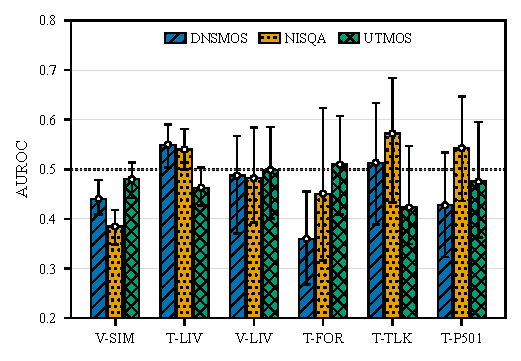
\includegraphics[width=\columnwidth]{figures/auroc_bar.pdf}
  \vspace{-.8cm}
  \caption{Within-domain detection of the highest absolute-error quartile using Mahalanobis distance. Color and hatch encode the predictor. Points show AUROC estimates and error bars show group-bootstrap 95\% confidence intervals from 2{,}000 resamples. V-SIM is included because this is error detection rather than domain discrimination. %The dotted line denotes chance performance.
  }
  \label{fig:error-auroc}
\end{figure}

Figure~\ref{fig:error-auroc} shows that domain discrimination and error detection are not interchangeable. Across the 18 predictor--subset pairs, mean error-detection AUROC is 0.478 for Mahalanobis distance. The corresponding means are 0.433 for Euclidean distance, 0.499 for nearest-neighbour distance, and 0.421 for prediction extremity $|\qhat-3|$. On T-LIV, Mahalanobis AUROC is 0.549 for DNSMOS, 0.540 for NISQA, and 0.463 for UTMOS. DNSMOS on T-FOR reaches only 0.360 with 95\% CI $[0.268,0.455]$, and NISQA on its own held-out V-SIM half reaches 0.385 with CI $[0.349,0.418]$, an equally sub-chance and even tighter interval on the model's in-sample data. Spearman correlation between $\dMx$ and $|\qhat-\qtrue|$ within each subset, a continuous rank-correlation check, agrees qualitatively with the AUROC-based conclusion: correlations are small and inconsistent in sign across predictors and subsets. A single higher-distance-means-higher-error rejection rule is therefore not transferable.

Applying the NISQA-Corpus-fitted Mahalanobis, Euclidean, and nearest-neighbour references, without refitting, to 364 clips from the Interspeech 2025 URGENT Challenge~\cite{Sach2025} (six languages, 26 enhancement systems) gives domain-detection AUROC up to 0.911 against held-out V-SIM but error-detection AUROC of only 0.415 to 0.541. This dissociation is not specific to NISQA Corpus.

\vspace{-.2cm}
\subsection{Conformal Intervals}
\label{ssec:interval-results}

Table~\ref{tab:coverage} reports the fixed and five-bin Mahalanobis-adaptive intervals. Fixed coverage on held-out V-SIM is 90.2\%, 90.1\%, and 91.8\% for DNSMOS, NISQA, and UTMOS. This confirms the expected in-domain behavior of the disjoint calibration design. Fixed widths span 2.26 to 2.91 MOS, 56--73\% of the four-point (1--5) scale, so the coverage guarantee is bought with intervals that occupy most of the usable range. Coverage under shift ranges from 66.4\% to 100.0\%, which is consistent with the absence of an arbitrary-shift guarantee.

Adaptation is predictor and domain dependent. For NISQA, coverage changes from 97.1\% to 90.4\% on T-P501 and from 93.5\% to 84.1\% on T-TLK. Both changes have bootstrap CIs that exclude zero. $k$-NN and Euclidean bins avoid this T-TLK undercoverage. The evidence does not support a better wrapper.